\documentclass[12pt,fleqn]{article}\usepackage{../common}
\begin{document}
\textbf{Log Lineer Modeller ve Kosulsal Rasgele Alanlar (Log Linear Models and
Conditional Random Fields)}

Ders 2

Charles Elkan ders notlari

Kosulsal Olurluk (Conditional Likelihood)

Diyelim ki elimizde egitim verisi olarak ikili $<x,y>$ veri noktalari
var. O zaman $y$'nin $x$'e kosulsal olarak bagli (conditional on) bir
dagilimi oldugunu soyleyebiliriz. 

$$ y \sim f(x;\theta) $$

Yani her $x$ icin farkli bir $y$ dagilimi ortaya cikabilir. Ve tum bu
farkli dagilimlarin ortak noktasi $\theta$ parametresidir. Kosulsal
olasilik yani soyle yazilabilir, 

$$ P(Y=y | X=x;\theta) $$

Usttekiler $Y$ icin bir model ortaya koydu, peki elimizde $X$'in dagilimi
icin bir olasilik modelimiz var mi? Cevap hayir. Niye? Dusunelim, $p(y,x)$
nedir ?

$$ p(x,y) = p(x)p(y|x) $$

Ustte $p(y|x)$'i tanimlayacak ($\theta$ uzerinden) bir olasilik demeti /
ailesi tanimladik, fakat elimizde $p(x)$ dagilimini verecek bir model
yok, o zaman $p(x,y)$'yi tanimlayacak bir model de yok.

Fakat bu dunyanin sonu degil. Belki de Makine Ogrenimi bransinin bir
slogani su olmali: ``Ogrenmen gerekmeyen seyi ogrenme''. Ustteki ornekte
$p(y|x)$'i ogrenebiliriz, ama $p(x)$'i illa ogrenmemiz gerekir mi?

Siniflayici (classifier) ve takip edilen (supervised) ogrenim durumunu
dusunursek, bize egitim amacli olarak $<x,y>$ ikili veri noktalari
saglanacak. $x$ kaynak veri, $y$ tahmin edilecek (ya da basta egitim hedefi
olan) etiket olacak. $y$ icin bir model ortaya cikartiyoruz, cunku test
zamaninda $y$ olmayacak, fakat $x$ hep olacak. Yani $y$'nin modellenmesi
mecburi, cunku ``genelleyerek'' onun ne oldugunu bulacagiz, ama $x$ hep
verili.

Kosulsal Olurluk Maksimum Olurluk Prensibi

Egitim verisi $<x_1,y_1>,...,<x_n,y_n>$ icin, $\theta$'yi soyle sec

$$ \hat{\theta} =  \arg\max_{\theta} \prod _{i=1}^{n} p(y_i | x_i;\theta) $$

Normal maksimum olurlukta bilindigi gibi olasiliklarin carpimi maksimize
edilir, burada maksimize ettigimiz ``kosulsal'' olasiliklarin carpimi. 

Burada onemli bir soru su: bildigimiz gibi maksimum olurluk hesabi her veri
noktasinin bir digerinden bagimsiz oldugunu farzeder [cunku her olurluk
hesabini bir diger ile carpiyoruz, baska ek carpim, toplama, vs
yapmiyoruz], bu faraziye dogru bir faraziye midir? Bu soru ve ona verilecek
cevap cok onemli. Evet, eger egitim noktalari birbirinden bagimsiz degilse
maksimum olurluk kullanmamaliyiz. Bagimsizligi da iyi tanimlamak gerekiyor
tabii, eger ustteki durumda $x_i$ {\em verildikten sonra} $y_i$'larin
birbirinden bagimsiz olmasi yeterli.

Bu model klasik Istatistik'te cokca kullanilan bir yaklasimdir, hatta
lineer regresyon'un temeli ustteki faraziyedir. 

$$ y = \alpha + \bar{\beta}\bar{x} + N(0,\sigma^2) $$

Bu standart lineer regresyon modeli, ve bu modelde her $y$ ona tekabul eden
$x$'e bagli, bu sayede $x$'ler biliniyorsa $y$'ler birbirinden kosulsal
olarak bagimsiz hale geliyor, boylece $x$'ler birbirine bagimli olsa bile
$\alpha$ ve $\beta$'nin bulunmasi mumkun oluyor. 

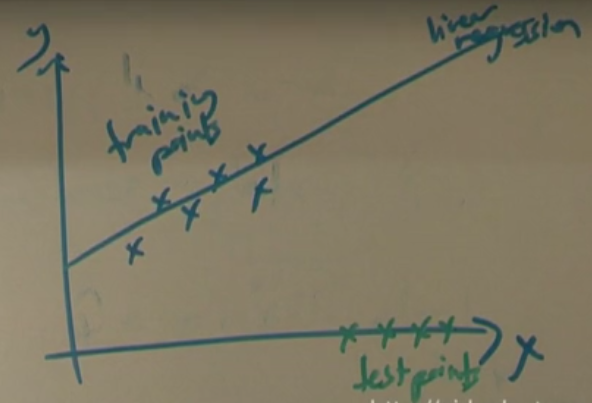
\includegraphics[height=4cm]{crf_1.png}

Ustteki resimde egitim noktalari (training points) mavi olsun, test
noktalari yesil olsun (hemen altinda). Bazi Yapay Ogrenim yaklasimlari
diyebilir ki egitim $x$'lerinin dagilimi test $x$'lerinin dagilimindan
farkli, bu veri seti ogrenilemez (yani genellenemez, modellenemez). Fakat
klasik Istatistik buna bakar ve der ki $x$'lerin verildigi durumda $y$'ler
bagimsizdir, bu sekilde bir kosulsal model ogrenilebilir.

Lojistik Regresyon ayni sekilde isler (lojistik regresyon, log lineer
modellerin ozel bir halidir, Kosulsal Rasgele Alanlar ayni sekilde). Burada
da ogrenilen bir

$$ p = p(y | x;\alpha,\beta) $$

modeli vardir ve $y$ degerleri sadece 0 ve 1 olabilir. Tahmin edilen
olasilik ise $y$'nin 1 olma olasiligidir. Bu model Rasgele Gradyan Cikisi
ile egitilir [detaylar icin {\em Lojistik Regresyon} notlarimiza
bakabilirsiniz].

$$ log \frac{p}{1-p} = \alpha + \sum_j \beta_j x_j $$

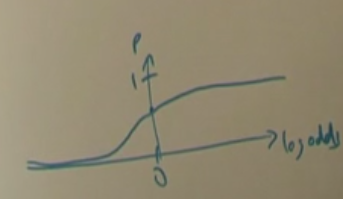
\includegraphics[height=4cm]{crf_2.png}

$p$ log sansinin monotonik bir fonksiyonudur, ve ters yonden bakarsak, log
sans $p$'nin monotonik bir fonksiyonudur. Yani lineer bir fonksiyon (sag
taraf) ne kadar buyurse, olasilik / log sans o kadar buyuyecektir. Bu
buyume durumu mesela $\beta_j$ katsayisini veri analizi baglaminda
yorumlanabilir hale getirir. Diyelim ki $\beta_4$ katsayisi pozitif, o
zaman diger tum sartlarin esit oldugu durumda (with all else being equal)
$x_4$ ne kadar buyurse 1 olma olasiligi o kadar artar.

Lojistik modellerin onemli bazi avantajlari var, ki bu avantajlar log
lineer modellere de sirayet ediyor (bu iyi). 

1) Degiskenler arasi ilinti (correlation) probleme yol acmaz: Bu fayda
aslinda daha once belirttigimiz $x$'lerin birbirine bagimli olabilmesi ile
alakali. Bagimsizlik onsarti aranmadigi icin istedigimiz kadar $x$'i
problemin uzerine atabiliriz, egitici algoritma bunlardan cikartabildigi
kadar iyi bir model bulacaktir.

Kiyasla mesela Naive Bayes boyle degildir, eger bir NB siniflayicisini
egitiyorsak, ve ogelerin (feature) arasinda ilinti var ise, siniflayicinin
dogrulugu (accuracy) azalabilir.

2) LR ile ``1 olma olasiligini'', yani ``bir sayisal skoru'', elde
ediyoruz, bu sadece 1/0 degerinden daha fazla bir bilgi demektir.

3) Bu skor, anlami olan bir olasiliksal degerdir: Sonucta SVM
siniflayicilari da $-\infty$ ve $+\infty$ arasinda degerler dondururler, ve
bu degerler siralama (ranking) amacli kullanilabilir, fakat olasilik
matematigi acisindan anlami olan bir degerin olmasi bundan bile
iyidir. Naive Bayes 0 ve 1 arasinda deger dondurebilir, fakat bu degerlerin
de olasiliksal olarak aslinda anlami yoktur, pratikte goruldu ki bu
degerler cok uc noktalarda, ya sifira cok yakin, ya bire cok
yakin. Literaturde NB skorlarinin ``iyi kalibre edilmis olmadigi''
soylenir.

$X_1,...,X_n$ test ornekleri ve tahmin edilen olasiliklar $P(Y=1 | x_i) =
v_i$
olsun. Diyelim ki $s = \sum_i v_i$ ve $t$ sayisi $1,..,n$ tane ogenin
icinden $y = 1$ degerini tasiyan ogelerin sayisi olsun. Ornek, elimizde 100
tane egitim noktasi var, bunlarin 60'i 1 degerinde. Bu durumda $s$ yaklasik
60 olacaktir (rasgele gurultuyu hesaba katarsak tabii), yani  $E[t] =
s$ 
denebilecektir ve bu sadece eger olasiliklar iyi kalibre edilmisse
soylenebilir.

4) Dengesiz egitim verisi kullanilabilir: pek cok egitim setinde mesela 1
degeri tasiyan degerleri 0 degeri tasiyanlardan cok daha fazla. Lojistik
regresyon bu tur veriyle rahatca calisabilir.
 
Ders 3

Lojistik regresyon icin log olurlugun (LCL) turevini almak lazim. Once
basitlestirme amacli $\alpha = \beta_o$, ve $x_0 = 1$. O zaman log sansin
eski hali (altta esitligin sol tarafi) soyle yazilabilir (sag taraf), daha
derli toplu bir formul olur,

$$ \alpha + \sum_j \beta_j x_j  = \sum_{j=0}^{d} \beta_j x_j $$ 

Bulmak istedigim her $j$ icin $\frac{d}{d\beta_j} LCL$ lazim

$$ 
\frac{d}{d\beta_j} LCL = 
\sum _{i:y_i=1} \frac{d}{d\beta_j} \log p(1|..)
+ \sum _{i:y_i=0} \frac{d}{d\beta_j} \log p(0|..)
\ \ \ (3)
$$

Eger ustteki bir bolumu $p$ digerine $1-p$ dersem, yani soyle

$$ 
= \sum _{i:y_i=1} \frac{d}{d\beta_j} \underbrace{\log p(1|..)}_{p}
+ \sum _{i:y_i=0} \frac{d}{d\beta_j} \underbrace{\log p(0|..)}_{1-p}
$$

O zaman 


$$ 
= \sum _{i:y_i=1} \frac{d}{d\beta_j}\log p
+ \sum _{i:y_i=0} \frac{d}{d\beta_j} \log (1-p)
$$
Biliyoruz ki

$$ 
\frac{d}{d\beta_j}\log p = \frac{1}{p}\frac{d}{d\beta_j} p
\ \ \ (1)
$$

$$ 
\frac{d}{d\beta_j}\log (1-p) = \frac{1}{1-p}(-1)\frac{d}{d\beta_j} p
\ \ \ (2)
$$

Ustteki son iki formulun her ikisinde de $d/d\beta_j p$ kismi olduguna dikkat.

Notasyon

$$ e = \exp \big[ - \sum_{j=0}^n \beta_jx_j \big] $$

$$ p = \frac{ 1}{1+e} $$

$$ 1-p = \frac{ 1+e-1}{1+e} = \frac{ e}{1+e} $$

Simdi  $d/d\beta_j p$'e donelim, ve $p$'nin ustteki gibi oldugundan
hareketle,

$$ \frac{ d}{d\beta_j}p = (-1)(1+e)^{-2} \frac{ d}{d\beta_j}e $$


$$ = (-1)(1+e)^{-2} (e) \frac{ d}{d\beta_j}(x_j) $$

$$ = \frac{ 1}{1+e} \frac{ e}{1+e}x_j = p(1-p)x_j$$


Son ifade kodlama icin oldukca uygun, $d/d\beta_j p$ hesabini yine icinde
$p$ iceren bir ifadeye bagladik, ayrica turev $x_j$ ile orantili. 

Bu hesapla aslinda (1) icindeki $d/d\beta_j p$ kismini hesaplamis
olduk. Eger yerine koyarsak, 

$$ 
\frac{d}{d\beta_j}\log p = \frac{1}{p}p(1-p)x_j 
$$

$p$'ler iptal olur

$$ 
= (1-p)x_j 
$$

Ayni sekilde (2) icin 

$$ 
\frac{d}{d\beta_j}\log (1-p) = \frac{1}{1-p}(-1) p(1-p)x_j 
$$

$$ 
 =  -px_j 
$$


Ustteki turevler tek bir egitim veri noktasi icin. Tum egitim veri setinin
turevi her noktanin turevlerinin toplami olacak, (3)'de goruldugu gibi.

$$ \frac{d}{d\beta_j} LCL = 
\sum _{i: y_i = 1} (1-p_i)x_{ij} + 
\sum _{i: y_i = 0} -p_i x_{ij}  
\ \ \ (4)
$$

$x_{ij}$ notasyonunda $j$, $j^{inci}$ oge / ozellik anlamina geliyor. Simdi notasyonel bir numara kullanacagim, 

$$ = \sum _{tum \ i} (y_i - p_i)x_{ij} $$

Bunu niye yaptim? (4) formulunde esitligin sag tarafi, birinci terim icinde
1 sayisi var, sonraki terimde 1 yok. Eger 1 olup olmamasi yerine $y_i$
kullanirsam, ki zaten 1'in olup olmamasi $y_i$'nin 1 olup olmamasina bagli,
tek bir terimde isi halledebilirim. $y_i=1$ oldugu zaman ustteki ifade
$1-p_i$ olacaktir, olmadigi zaman $-p_i$ olacaktir. 

Eristigimiz sonucu analiz etmemiz gerekirse, nihai formul gayet basit ve
temiz cikti. 

[24:10] kalibrasyonla alakali bir yorum

Rasgele Gradyan Cikisi (Stochastic Gradient Ascent)

Fikir: turevi egitim noktasi basina hesapla, ve modeli hemen guncelle. 

Egitim noktalari $<x,y>$ olarak gelsinler. Her nokta icin, ve her $\beta_j$
icin

$$ \frac{d}{d\beta_j}p(y|x;\beta) = g_j$$ hesapla. 

$$ \beta_j := \beta_j + \alpha g_j $$

Gradyanin ne oldugunu hatirlayalim, bir fonksiyonun maksimumuna ``dogru''
olan bir gidis yonunu gosterir, ve bu gidis yonu o fonksiyonu olusturan
degiskenlerin (parcali turevleri) uzerinden belirtilir. O zaman elimizdeki
gradyan o ic degiskenlerin maksimum yondeki degisim seklini bize tarif
eder. 

Algoritmanin tamami: alttaki formul icin

$$ \frac{d}{d\beta_j}p(y|\bar{x};\bar{\beta}) = (y-p)x_j $$

Her $x$ icin

- O anki modele gore $p$'yi hesapla

- Her $j = 0,..,d$ icin

\ \ \ - $ \beta_j := \beta_j + \alpha \underbrace{ (y-p) x_j}_{kismi \ turev} $ hesapla
  
Peki metotun ismindeki ``rasgele (stochastic)'' tanimi nereden geliyor? Iyi
bir soru bu cunku metotta rasgele sayi uretimi gibi seyler
gormuyoruz. Cevap, metot yine de rasgele, cunku her noktayi ayri ayri
isliyoruz, ve bu noktalarin egitim algoritmasini gelisi bir nevi ``veriyi
orneklemek'' gibi sanki, ek olarak veriyi egitime almadan once rasgele
sekilde karistirmak ta iyi olabilir. 

Bazi Tavsiyeler (Heuristics)

1) Her ozellik (feature) $x_j$'i olceklemek, yani ayni ortalama (mean) ve
varyansa sahip olacak sekilde tekrar ayarlamak. Yani mesela 0 ile 100
arasinda olabilecek ``yas'' gibi bir ozelligi, 0 ve 1 arasinda degisen
ozellikler ile ayni ortalama ve varyansa sahip olacak sekilde
ayarlamak. Bunun sebebi guncelleme hesabindaki $\lambda$'nin tek bir sabit
olmasi, ve bu sabit her $j$ icin aynidir, o sebeple $\lambda$'nin her ogeye
``ayni sekilde'' uygulanabilmesi icin ogelerin birbirine yakin olmasi
iyidir. Ek olarak, genellikle egitim verisinde 0 ile 1 arasinda ikisel
turden ogeler vardir, o sebeple bu sekilde olmayan diger ogeleri 0 ve 1
arasinda cekmek daha uygun ve kolay olur.

2) Veriyi rasgele sekilde siralamak. Terminoloji: egitim veri seti
uzerinden bir gecis yapmak bir ``cag'' (epoch) olarak bilinir. 

3) $\lambda$'yi deneme / yanilma yontemi ile bulun (bu sabiti bulmanin
sistemik bir yontemi yok). Belki verinin icinden alinan daha ufak bir
orneklem uzerinde bu deneme / yanilma islemi yapilabilir.



















\end{document}
